%!TEX program = xelatex
% Encoding: UTF8
% SEIKA 2015


% Chapter 2 TutorialsHow to ...
% Section 2.2

\newpage
\section {MNIST机器学习入门}\label{MINIST_beginner}

Ⓔ \textcolor{etc}{This tutorial is intended for readers who are new to both machine learning and TensorFlow. If you already know what MNIST is, and what softmax (multinomial logistic) regression is, you might prefer this faster paced tutorial. Be sure to install TensorFlow before starting either tutorial.}

Ⓒ 本教程的目标读者是对机器学习和TensorFlow都不太了解的新手.如果你已经了解MNIST和softmax回归(softmax regression)的相关知识,你可以阅读这个快速上手教程.

Ⓔ \textcolor{etc}{When one learns how to program, there's a tradition that the first thing you do is print "Hello World." Just like programming has Hello World, machine learning has MNIST.}

Ⓒ 当我们开始学习编程的时候,第一件事往往是学习打印“Hello World”.就好比编程入门有Hello World,机器学习入门有MNIST.\index{MNIST 数据集}

Ⓔ \textcolor{etc}{MNIST is a simple computer vision dataset. It consists of images of handwritten digits like these:}

Ⓒ MNIST是一个入门级的计算机视觉数据集,它包含各种手写数字图片:

\begin{figure}[htbp]
\centering
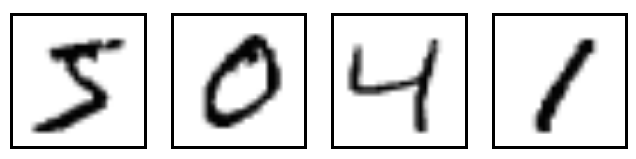
\includegraphics[width=.55\textwidth]{../SOURCE/images/MNIST.png}
\caption{}
\end{figure}

Ⓔ \textcolor{etc}{It also includes labels for each image, telling us which digit it is. For example, the labels for the above images are 5, 0, 4, and 1.}

Ⓒ 它也包含每一张图片对应的标签,告诉我们这个是数字几.比如,上面这四张图片的标签分别是5,0,4,1.

Ⓔ \textcolor{etc}{In this tutorial, we're going to train a model to look at images and predict what digits they are. Our goal isn't to train a really elaborate model that achieves state-of-the-art performance -- although we'll give you code to do that later! -- but rather to dip a toe into using TensorFlow. As such, we're going to start with a very simple model, called a Softmax Regression.}

Ⓒ 在此教程中,我们将训练一个机器学习模型用于预测图片里面的数字.我们的目的不是要设计一个世界一流的复杂模型---尽管我们会在之后给你源代码去实现一流的预测模型---而是要介绍下如何使用TensorFlow.所以,我们这里会从一个很简单的数学模型开始,它叫做Softmax Regression.

Ⓔ \textcolor{etc}{The actual code for this tutorial is very short, and all the interesting stuff happens in just three lines. However, it is very important to understand the ideas behind it: both how TensorFlow works and the core machine learning concepts. Because of this, we are going to very carefully work through the code.}

Ⓒ 对应这个教程的实现代码很短,而且真正有意思的内容只包含在三行代码里面.但是,去理解包含在这些代码里面的设计思想是非常重要的:TensorFlow工作流程和机器学习的基本概念.因此,这个教程会很详细地介绍这些代码的实现原理.

\subsection {The MNIST Data  |  MNIST数据集}

Ⓔ \textcolor{etc}{The MNIST data is hosted on Yann LeCun's website. For your convenience, we've included some python code to download and install the data automatically. You can either download the code and import it as below, or simply copy and paste it in.}

Ⓒ MNIST数据集的官网是\href{http://yann.lecun.com/exdb/mnist/}{Yann LeCun's website}.在这里,我们提供了一份python源代码用于自动下载和安装这个数据集.你可以下载这段\href{https://tensorflow.googlesource.com/tensorflow/+/master/tensorflow/examples/tutorials/mnist/input_data.py}{代码},然后用下面的代码导入到你的项目里面,也可以直接复制粘贴到你的代码文件里面.


%\begin{lstlisting}[language={[ANSI]Python}]
\begin{lstlisting}
import input_data
mnist = input_data.read_data_sets("MNIST_data/", one_hot=True)
\end{lstlisting}

Ⓔ \textcolor{etc}{The downloaded data is split into three parts, 55,000 data points of training data \lstinline{(mnist.train)}, 10,000 points of test data \lstinline{(mnist.test)}, and 5,000 points of validation data \lstinline{(mnist.validation)}. This split is very important: it's essential in machine learning that we have separate data which we don't learn from so that we can make sure that what we've learned actually generalizes!}

Ⓒ 下载下来的数据集可被分为三部分:55000 行训练用点数据集(\lstinline{mnist.train}),10000 行测试数据集(\lstinline{mnist.test}),以及5000行验证数据集(\lstinline{mnist.validation}).这样的切分很重要:在机器学习模型设计时必须有一个单独的测试数据集不用于训练而是用来评估这个模型的性能,从而更加容易把设计的模型推广到其他数据集上(泛化).

Ⓔ \textcolor{etc}{As mentioned earlier, every MNIST data point has two parts: an image of a handwritten digit and a corresponding label. We will call the images "xs" and the labels "ys". Both the training set and test set contain xs and ys, for example the training images are \lstinline{mnist.train.images} and the train labels are \lstinline{mnist.train.labels}.}

Ⓒ 正如前面提到的一样,每一个MNIST数据单元有两部分组成:一张包含手写数字的图片和一个对应的标签.我们把这些图片设为“xs”,把这些标签设为“ys”.训练数据集和测试数据集都包含xs和ys,比如训练数据集的图片是\lstinline{mnist.train.images} ,训练数据集的标签是\lstinline{mnist.train.labels}.

Ⓔ \textcolor{etc}{Each image is 28 pixels by 28 pixels. We can interpret this as a big array of numbers:}

Ⓒ 每一张图片包含$ 28 \times 28$像素.我们可以用一个数字数组来表示这张图片:

\begin{figure}[htbp]
\centering
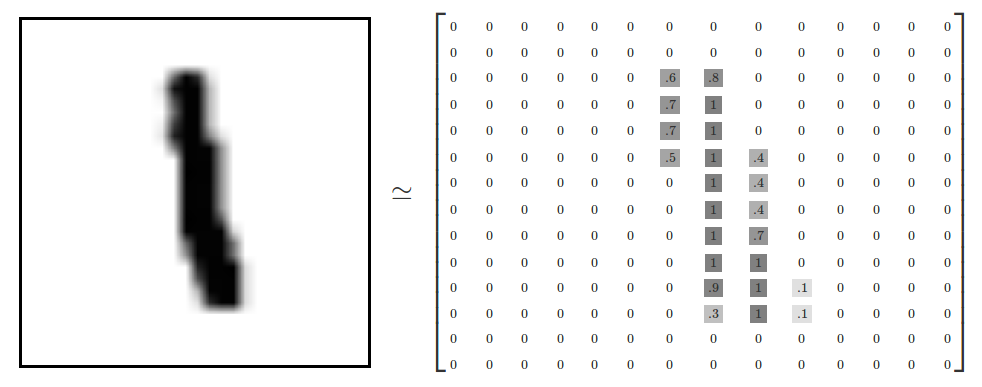
\includegraphics[width=.8\textwidth]{../SOURCE/images/MNIST-Matrix.png}
\caption{}
\end{figure}

Ⓔ \textcolor{etc}{We can flatten this array into a vector of $ 28 \times 28 = 784$ numbers. It doesn't matter how we flatten the array, as long as we're consistent between images. From this perspective, the MNIST images are just a bunch of points in a 784-dimensional vector space, with a \href{http://colah.github.io/posts/2014-10-Visualizing-MNIST/}{very rich structure} (warning: computationally intensive visualizations).}

Ⓒ 我们把这个数组展开成一个向量,长度是 $ 28 \times 28 = 784$.如何展开这个数组(数字间的顺序)不重要,只要保持各个图片采用相同的方式展开.从这个角度来看,MNIST数据集的图片就是在784维向量空间里面的点, 并且拥有比较\href{http://colah.github.io/posts/2014-10-Visualizing-MNIST/}{复杂的结构} (注意: 此类数据的可视化是计算密集型的).

Ⓔ \textcolor{etc}{Flattening the data throws away information about the 2D structure of the image. Isn't that bad? Well, the best computer vision methods do exploit this structure, and we will in later tutorials. But the simple method we will be using here, a softmax regression, won't.}

Ⓒ 展平图片的数字数组会丢失图片的二维结构信息.这显然是不理想的,最优秀的计算机视觉方法会挖掘并利用这些结构信息,我们会在后续教程中介绍.但是在这个教程中我们忽略这些结构,所介绍的简单数学模型,softmax回归(softmax regression),不会利用这些结构信息.

Ⓔ \textcolor{etc}{The result is that \lstinline{mnist.train.images} is a tensor (an n-dimensional array) with a shape of \lstinline{[55000, 784]}. The first dimension indexes the images and the second dimension indexes the pixels in each image. Each entry in the tensor is the pixel intensity between 0 and 1, for a particular pixel in a particular image.}

Ⓒ 因此,在MNIST训练数据集中,\lstinline{mnist.train.images}是一个形状为 \lstinline{[55000, 784]} 的张量,第一个维度数字用来索引图片,第二个维度数字用来索引每张图片中的像素点.在此张量里的每一个元素,都表示某张图片里的某个像素的强度值,值介于0和1之间.

\begin{figure}[htbp]
\centering
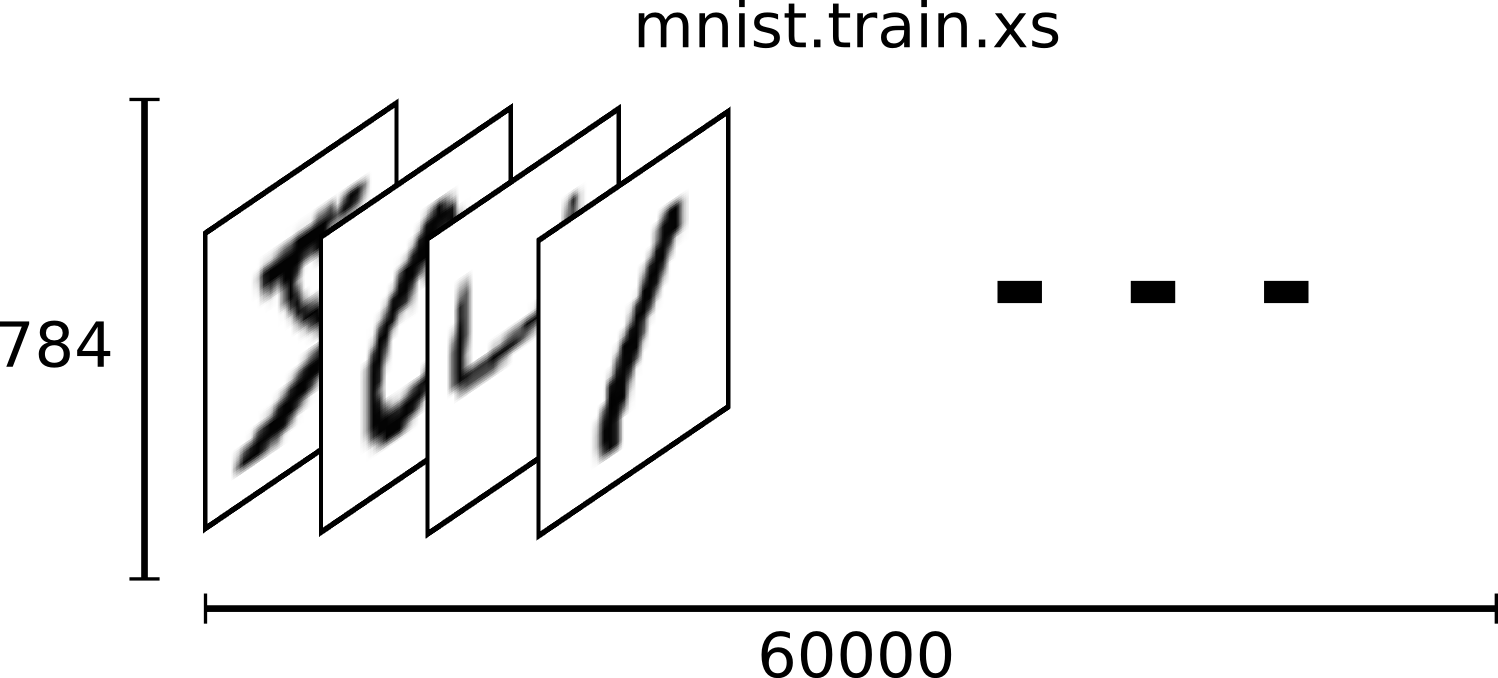
\includegraphics[width=.65\textwidth]{../SOURCE/images/mnist-train-xs.png}
\caption{}
\end{figure}

Ⓔ \textcolor{etc}{The corresponding labels in MNIST are numbers between 0 and 9, describing which digit a given image is of. For the purposes of this tutorial, we're going to want our labels as "one-hot vectors". A one-hot vector is a vector which is 0 in most dimensions, and 1 in a single dimension. In this case, the $n$th digit will be represented as a vector which is 1 in the $n$th dimensions. For example, 3 would be $[0,0,0,1,0,0,0,0,0,0]$. Consequently, \lstinline{mnist.train.labels} is a \lstinline{[55000, 10]} array of floats.}

Ⓒ 相对应的MNIST数据集的标签是介于0到9的数字,用来描述给定图片里表示的数字.为了用于这个教程,我们使标签数据是"one-hot vectors". 一个one-hot向量除了某一位的数字是1以外其余各维度数字都是0.所以在此教程中,数字n将表示成一个只有在第$n$维度(从0开始)数字为1的10维向量.比如,标签3将表示成(\lstinline{[0,0,0,1,0,0,0,0,0,0]}).因此,\lstinline{mnist.train.labels}是一个 \lstinline{[55000, 10]} 的数字矩阵.

\begin{figure}[htbp]
\centering
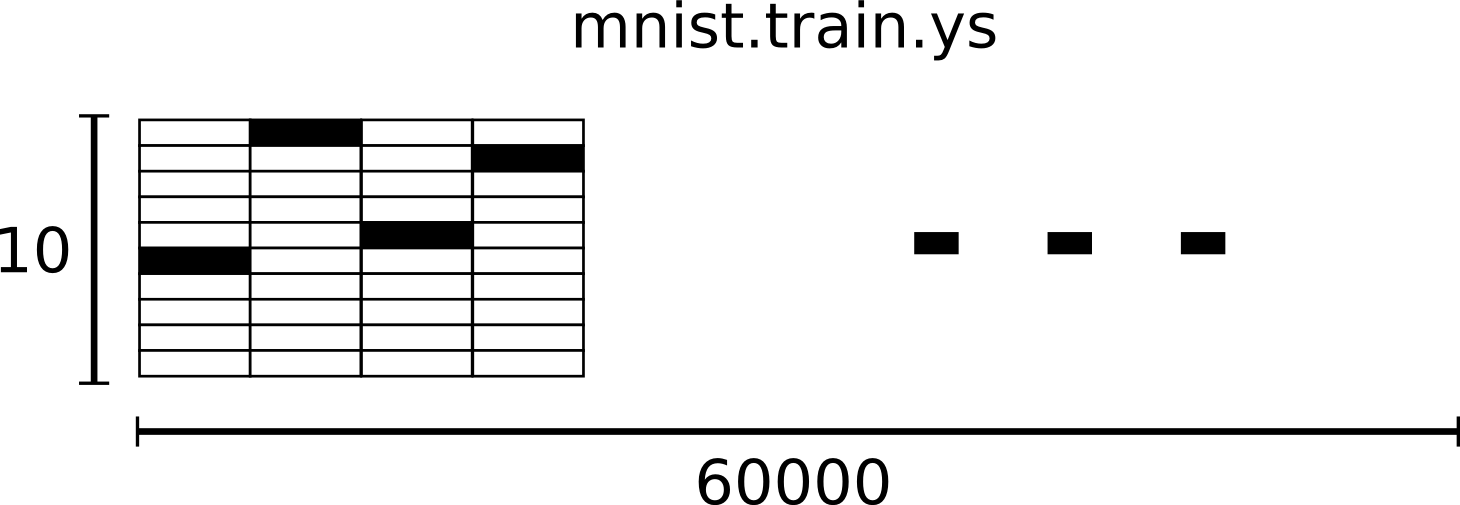
\includegraphics[width=.7\textwidth]{../SOURCE/images/mnist-train-ys.png}
\caption{}
\end{figure}

Ⓔ \textcolor{etc}{We're now ready to actually make our model!}

Ⓒ 现在,我们准备开始真正的建模之旅!

\subsection {Softmax回归介绍}

Ⓔ We know that every image in MNIST is a digit, whether it's a zero or a nine. We want to be able to look at an image and give probabilities for it being each digit. For example, our model might look at a picture of a nine and be 80\% sure it's a nine, but give a 5\% chance to it being an eight (because of the top loop) and a bit of probability to all the others because it isn't sure.

Ⓒ 我们知道MNIST数据集的每一张图片都表示一个(0到9的)数字.那么,如果模型若能看到一张图就能知道它属于各个数字的对应概率就好了。比如,我们的模型可能看到一张数字"9"的图片,就判断出它是数字"9"的概率为80\%,而有5\%的概率属于数字"8"(因为8和9都有上半部分的小圆),同时给予其他数字对应的小概率(因为该图像代表它们的可能性微乎其微).\index{Softmax regression}

Ⓔ This is a classic case where a softmax regression is a natural, simple model. If you want to assign probabilities to an object being one of several different things, softmax is the thing to do. Even later on, when we train more sophisticated models, the final step will be a layer of softmax.

Ⓒ 这是能够体现softmax回归自然简约的一个典型案例.softmax模型可以用来给不同的对象分配概率.在后文,我们训练更加复杂的模型时,最后一步也往往需要用softmax来分配概率.

Ⓔ A softmax regression has two steps: first we add up the evidence of our input being in certain classes, and then we convert that evidence into probabilities.

Ⓒ softmax回归(softmax regression)分两步:首先对输入被分类对象属于某个类的“证据”相加求和,然后将这个“证据”的和转化为概率.

Ⓔ To tally up the evidence that a given image is in a particular class, we do a weighted sum of the pixel intensities. The weight is negative if that pixel having a high intensity is evidence against the image being in that class, and positive if it is evidence in favor.

Ⓒ 我们使用加权的方法来累积计算一张图片是否属于某类的“证据”。如果图片的像素强有力的体现该图不属于某个类,则权重为负数,相反如果这个像素拥有有利的证据支持这张图片属于这个类,那么权值为正.

Ⓔ The following diagram shows the weights one model learned for each of these classes. Red represents negative weights, while blue represents positive weights.

Ⓒ 下面的图片显示了一个模型学习到的图片上每个像素对于特定数字类的权值.红色代表负权值,蓝色代表正权值.

\begin{figure}[htbp]
\centering
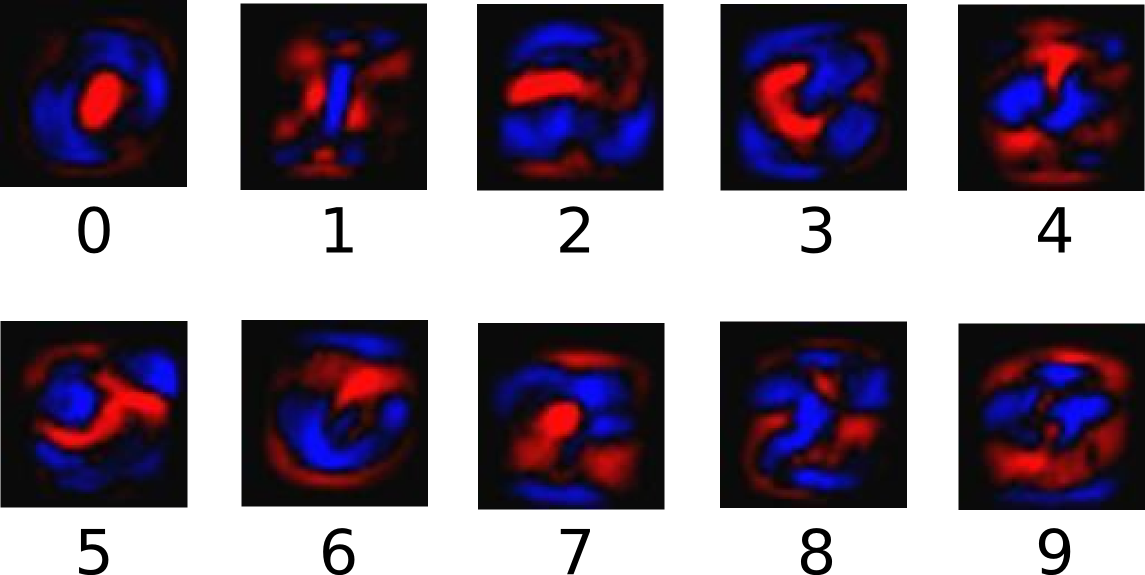
\includegraphics[width=.65\textwidth]{../SOURCE/images/softmax-weights.png}
\caption{}
\end{figure}

Ⓔ We also add some extra evidence called a bias. Basically, we want to be able to say that some things are more likely independent of the input. The result is that the evidence for a class $i$ given an input $x$ is:

Ⓒ 我们也需要引入额外的“证据”,可称之为偏置量(bias)。总的来说,我们希望它代表了与所输入向无关的判断证据.因此对于给定的输入图片$x$代表某数字$i$的总体证据可以表示为:
\begin{equation}
evidence_i = \sum_j{W_{i,j}}x_j+b_i
\end{equation}\\
Ⓔ where $W_i$ is the weights and $b_i$ is the bias for class $i$, and $j$ is an index for summing over the pixels in our input image $x$. We then convert the evidence tallies into our predicted probabilities y using the "softmax" function:\\
Ⓒ 其中,$W_i$ 代表权重,$b_i$ 代表第 $i$ 类的偏置量,$j$ 代表给定图片 $x$ 的像素索引用于像素求和.然后用softmax函数可以把这些证据转换成概率$y$:\\
\begin{equation}
y = softmax(evidence)
\end{equation}\\
Ⓔ Here softmax is serving as an "activation" or "link" function, shaping the output of our linear function into the form we want -- in this case, a probability distribution over 10 cases. You can think of it as converting tallies of evidence into probabilities of our input being in each class. It's defined as:\\
Ⓒ 这里的softmax可以看成是一个\emph{激励}(activation)函数或是\emph{链接}(link)函数,把我们定义的线性函数的输出转换成我们想要的格式,也就是关于10个数字类的概率分布.因此,给定一张图片,它对于每一个数字的吻合度可以被softmax函数转换成为一个概率值.softmax函数可以定义为:\\
\begin{equation}
softmax(x) = normalize(exp(x))
\end{equation}\\
Ⓔ If you expand that equation out, you get:\\
展开等式右边的子式,可以得到:\\
\begin{equation}
softmax(x)_i = \frac{exp(x_i)}{\sum_j{exp(x_j)}}
\end{equation}\\
Ⓔ But it's often more helpful to think of softmax the first way: exponentiating its inputs and then normalizing them. The exponentiation means that one more unit of evidence increases the weight given to any hypothesis multiplicatively. And conversely, having one less unit of evidence means that a hypothesis gets a fraction of its earlier weight. No hypothesis ever has zero or negative weight. Softmax then normalizes these weights, so that they add up to one, forming a valid probability distribution. (To get more intuition about the softmax function, check out the \href{http://neuralnetworksanddeeplearning.com/chap3.html#softmax}{section} on it in Michael Nieslen's book, complete with an interactive visualization.)\\
Ⓒ 但是更多的时候把softmax模型函数定义为第一种形式:把输入值当成幂指数求值,再正则化这些结果值.这个幂运算表示,更大的证据对应更大的假设模型(hypothesis)里面的乘数权重值.反之,拥有更少的证据意味着在假设模型里面拥有更小的乘数系数.假设模型里的权值不可以是0值或者负值.Softmax然后会正则化这些权重值,使它们的总和等于1,以此构造一个有效的概率分布.(更多的关于Softmax函数的信息,可以参考Michael Nieslen的书里面的\href{http://neuralnetworksanddeeplearning.com/chap3.html#softmax}{这个部分},其中有关于softmax的可交互式的可视化解释.)

Ⓔ You can picture our softmax regression as looking something like the following, although with a lot more $x$s. For each output, we compute a weighted sum of the $x$s, add a bias, and then apply softmax.\\
对于softmax回归模型可以用下面的图解释,对于输入的$xs$ 加权求和,再分别加上一个偏置量,最后再输入到softmax函数中:
\begin{center}
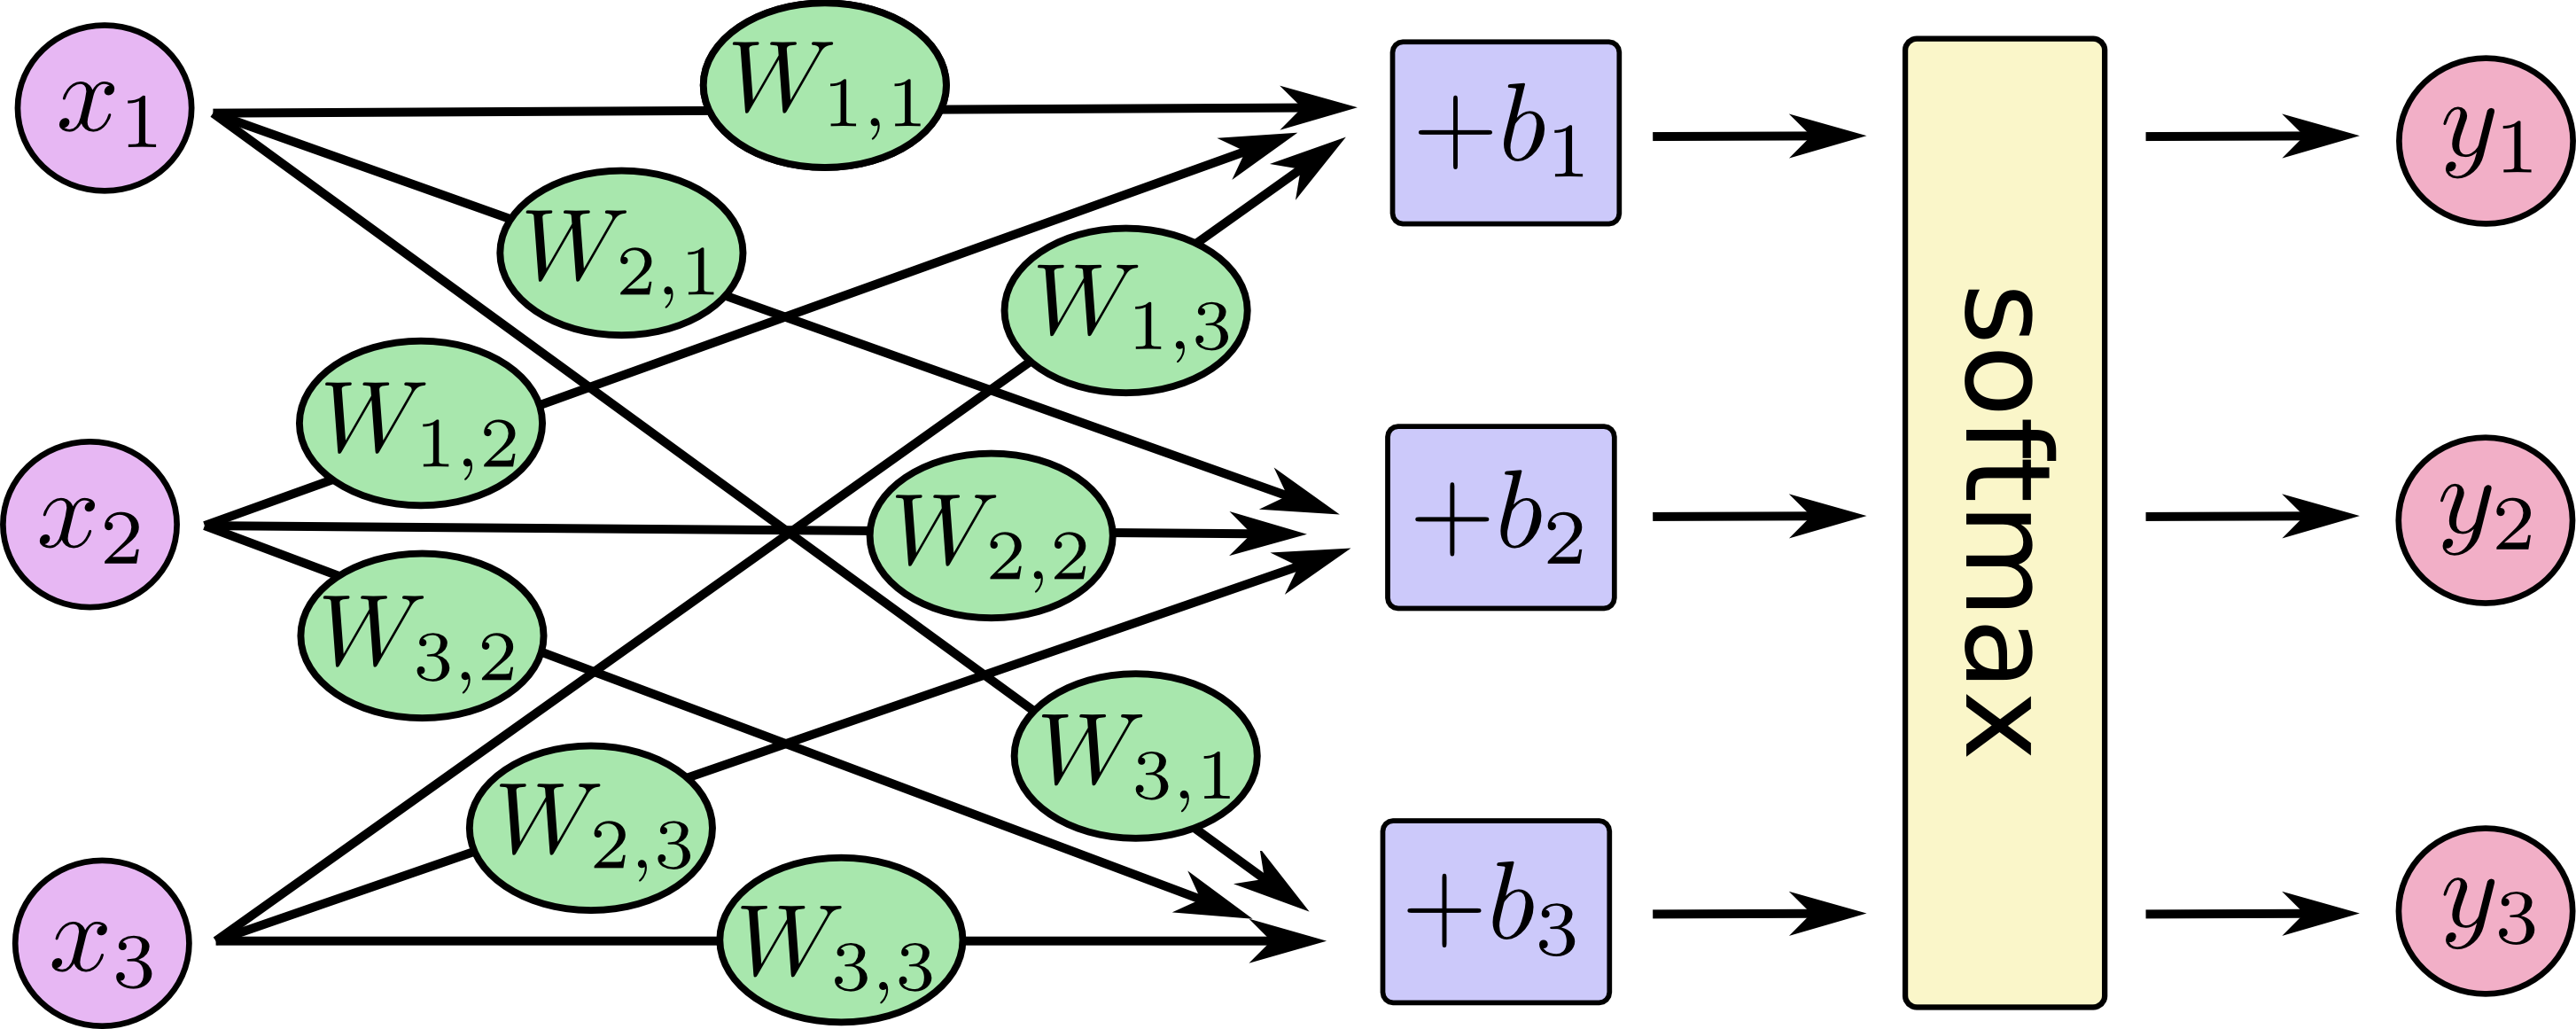
\includegraphics[width=.65\textwidth]{../SOURCE/images/softmax-regression-scalargraph.png}
\end{center}
Ⓔ If we write that out as equations, we get:\\
如果把它写成一个方程,可以得到:
\begin{center}
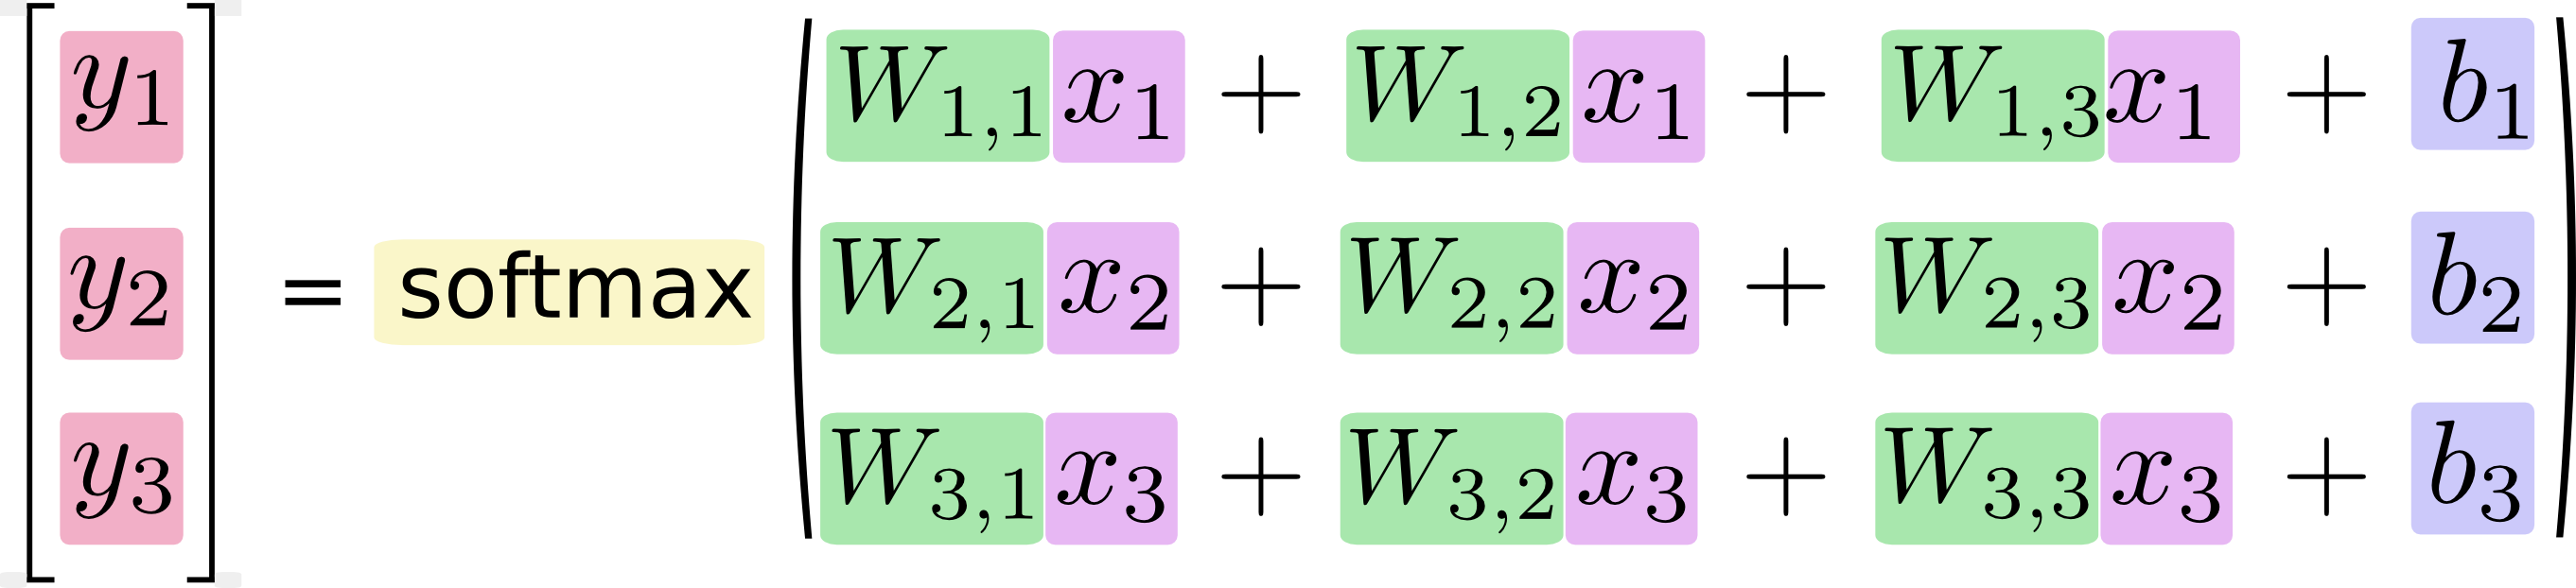
\includegraphics[width=.68\textwidth]{../SOURCE/images/softmax-regression-scalarequation.png}
\end{center}
Ⓔ We can "vectorize" this procedure, turning it into a matrix multiplication and vector addition. This is helpful for computational efficiency. (It's also a useful way to think.)\\
我们也可以用向量表示这个计算过程:用矩阵乘法和向量相加.这有助于提高计算效率(也是一种更有效的思考方式).
\begin{center}
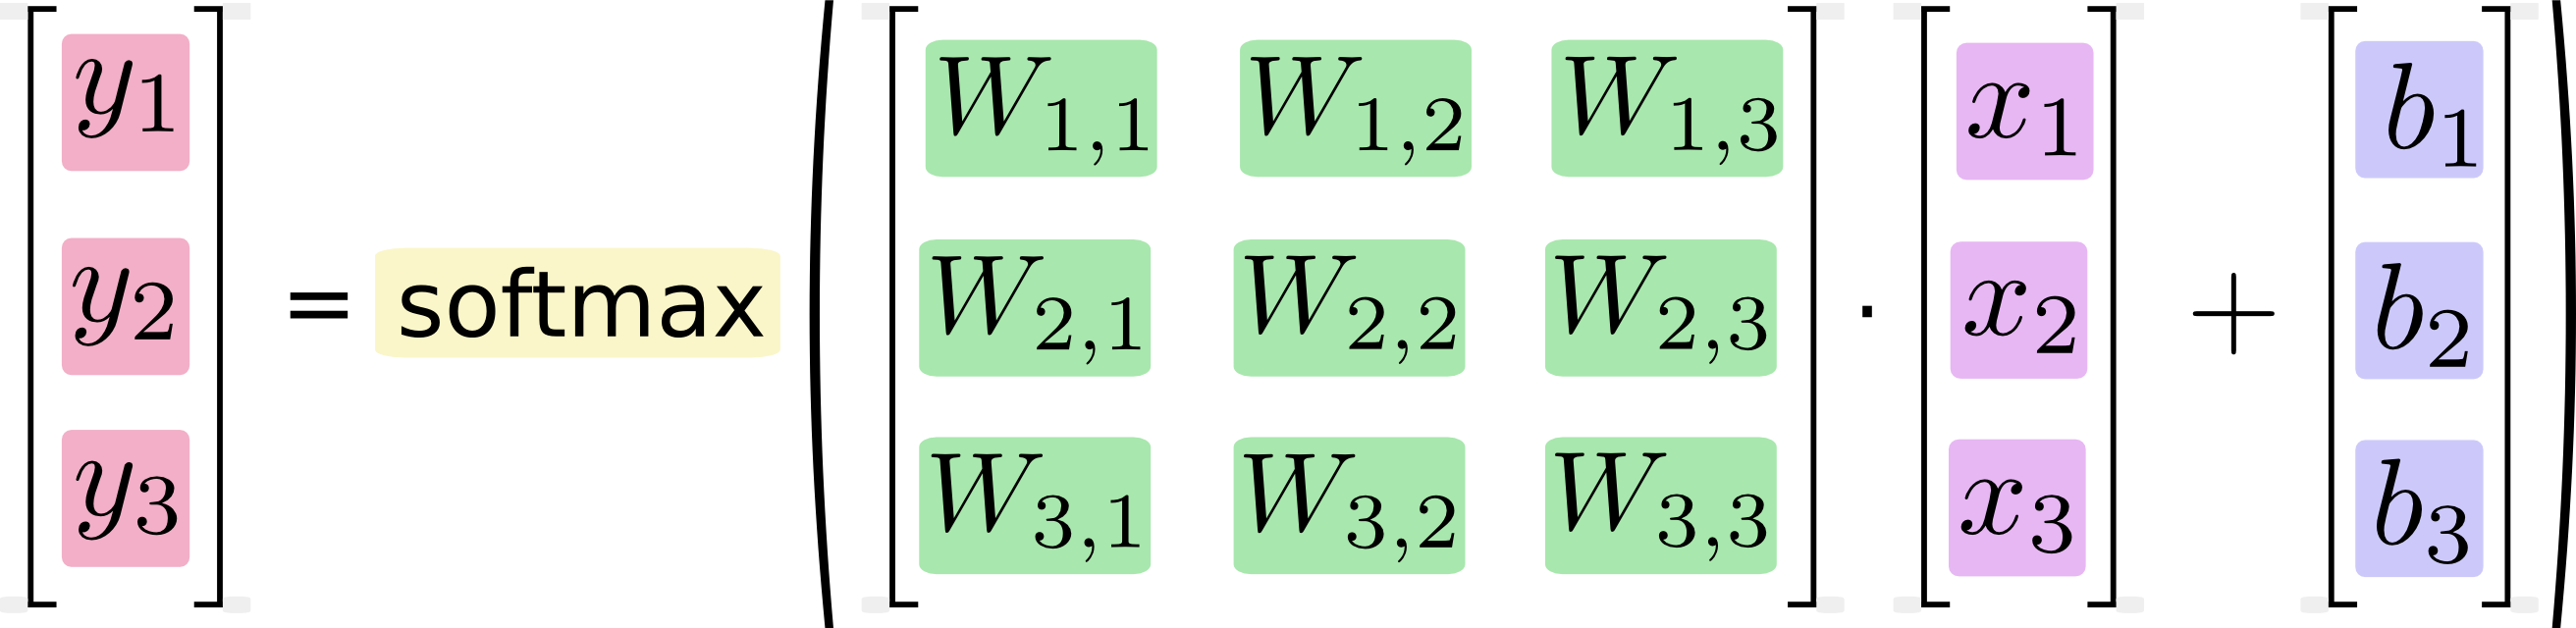
\includegraphics[width=.68\textwidth]{../SOURCE/images/softmax-regression-vectorequation.png}
\end{center}
Ⓔ More compactly, we can just write:\\
更进一步,可以写成更加紧凑的方式:
\begin{equation}
y = softmax(W_x+b)
\end{equation}

\subsection {实现回归模型}
Ⓔ To do efficient numerical computing in Python, we typically use libraries like NumPy that do expensive operations such as matrix multiplication outside Python, using highly efficient code implemented in another language. Unfortunately, there can still be a lot of overhead from switching back to Python every operation. This overhead is especially bad if you want to run computations on GPUs or in a distributed manner, where there can be a high cost to transferring data.

为了在python中高效的进行数值计算,我们通常会调用(如NumPy)外部函数库,把类似矩阵乘法这样的复杂运算使用其他外部语言实现.不幸的是,从外部计算切换回Python的每一个操作,仍然是一个很大的开销.如果你用GPU来进行外部计算,这样的开销会更大.用分布式的计算方式,也会花费更多的资源用来传输数据.

Ⓔ TensorFlow also does its heavy lifting outside python, but it takes things a step further to avoid this overhead. Instead of running a single expensive operation independently from Python, TensorFlow lets us describe a graph of interacting operations that run entirely outside Python. (Approaches like this can be seen in a few machine learning libraries.)

TensorFlow也把复杂的计算放在python之外完成,但是为了避免前面说的那些开销,它做了进一步完善.TensorFlow不单独地运行单一的复杂计算,而是让我们可以先用图描述一系列可交互的计算操作,然后全部一起在Python之外运行.(这样类似的运行方式,可以在不少的机器学习库中看到.)


Ⓔ To use TensorFlow, we need to import it.

使用TensorFlow之前,首先导入它:

\begin{lstlisting}
import tensorflow as tf
\end{lstlisting}

Ⓔ We describe these interacting operations by manipulating symbolic variables. Let's create one:

我们通过操作符号变量来描述这些可交互的操作单元,可以用下面的方式创建一个:

\begin{lstlisting}
x = tf.placeholder("float", [None, 784])
\end{lstlisting}\\
Ⓔ \lstinline{x} isn't a specific value. It's a \lstinline{placeholder}, a value that we'll input when we ask TensorFlow to run a computation. We want to be able to input any number of MNIST images, each flattened into a 784-dimensional vector. We represent this as a 2-D tensor of floating-point numbers, with a shape \lstinline{[None, 784]}. (Here None means that a dimension can be of any length.)\\
\lstinline{x} 不是一个特定的值,而是一个占位符\lstinline{placeholder},我们在TensorFlow运行计算时输入这个值.我们希望能够输入任意数量的MNIST图像,每一张图展平成784维的向量.我们用2维的浮点数张量来表示这些图,这个张量的形状是 [None,784].(这里的\lstinline{None}表示此张量的第一个维度可以是任何长度的.)


Ⓔ We also need the weights and biases for our model. We could imagine treating these like additional inputs, but TensorFlow has an even better way to handle it: \lstinline{Variable}. A \lstinline{Variable} is a modifiable tensor that lives in TensorFlow's graph of interacting operations. It can be used and even modified by the computation. For machine learning applications, one generally has the model parameters be \lstinline{Variables}.

我们的模型也需要权重值和偏置量,当然我们可以把它们当做是另外的输入(使用占位符),但TensorFlow有一个更好的方法来表示它们:\lstinline{Variable}. 一个\lstinline{Variable}代表一个可修改的张量,存在在TensorFlow的用于描述交互性操作的图中.它们可以用于计算输入值,也可以在计算中被修改.对于各种机器学习应用,一般都会有模型参数,可以用\lstinline{Variable}表示.

\begin{lstlisting}
W = tf.Variable(tf.zeros([784,10]))
b = tf.Variable(tf.zeros([10]))
\end{lstlisting}

Ⓔ We create these \lstinline{Variables} by giving \lstinline{tf.Variable} the initial value of the \lstinline{Variable}: in this case, we initialize both W and b as tensors full of zeros. Since we are going to learn \lstinline{W} and \lstinline{b}, it doesn't matter very much what they initially are.

我们赋予\lstinline{tf.Variable} 不同的初值来创建不同的\lstinline{Variable}:在这里,我们都用全为零的张量来初始化\lstinline{W}和\lstinline{b}.因为我们要学习\lstinline{W}和\lstinline{b}的值,它们的初值可以随意设置.


Ⓔ Notice that W has a shape of \lstinline{[784, 10]} because we want to multiply the 784-dimensional image vectors by it to produce 10-dimensional vectors of evidence for the difference classes. \lstinline{b} has a shape of \lstinline{[10]} so we can add it to the output.


注意,\lstinline{W}的维度是\lstinline{[784,10]},因为我们想要用784维的图片向量乘以它以得到一个10维的证据值向量,每一位对应不同数字类.\lstinline{b}的形状是\lstinline{[10]},所以我们可以直接把它加到输出上面.

Ⓔ We can now implement our model. It only takes one line!

现在,可以实现我们的模型了,只需以下一行代码:

\begin{lstlisting}
y = tf.nn.softmax(tf.matmul(x,W) + b)
\end{lstlisting}

Ⓔ First, we multiply $x$ by $W$ with the expression \lstinline{tf.matmul(x, W)}. This is flipped from when we multiplied them in our equation, where we had $W_x$, as a small trick to deal with x being a 2D tensor with multiple inputs. We then add b, and finally apply \lstinline{tf.nn.softmax}.

首先,我们用\lstinline{tf.matmul(X,W)}表示$x$乘以$W$,对应之前等式里面的$W_x$,这里$x$是一个2维张量拥有多个输入.然后再加上$b$,把和输入到\lstinline{tf.nn.softmax}函数里面.

Ⓔ That's it. It only took us one line to define our model, after a couple short lines of setup. That isn't because TensorFlow is designed to make a softmax regression particularly easy: it's just a very flexible way to describe many kinds of numerical computations, from machine learning models to physics simulations. And once defined, our model can be run on different devices: your computer's CPU, GPUs, and even phones!

至此,我们先用了几行简短的代码来设置变量,然后只用了一行代码来定义我们的模型.TensorFlow不仅仅可以使softmax回归模型计算变得特别简单,它也用这种非常灵活的方式来描述其他各种数值计算,从机器学习模型对物理学模拟仿真模型.一旦被定义好之后,我们的模型就可以在不同的设备上运行:计算机的CPU,GPU,甚至是手机!

\subsection{训练模型}

Ⓔ In order to train our model, we need to define what it means for the model to be good. Well, actually, in machine learning we typically define what it means for a model to be bad, called the cost or loss, and then try to minimize how bad it is. But the two are equivalent.

为了训练我们的模型,我们首先需要定义一个指标来评估这个模型是好的.其实,在机器学习,我们通常定义指标来表示一个模型是坏的,这个指标称为成本(cost)或损失(loss),然后尽量最小化这个指标.但是,这两种方式是相同的.

Ⓔ One very common, very nice cost function is "cross-entropy." Surprisingly, cross-entropy arises from thinking about information compressing codes in information theory but it winds up being an important idea in lots of areas, from gambling to machine learning. It's defined:\\
一个非常常见的,非常漂亮的成本函数是“交叉熵”(cross-entropy).交叉熵产生于信息论里面的信息压缩编码技术,但是它后来演变成为从博弈论到机器学习等其他领域里的重要技术手段.它的定义如下:
\\
\begin{equation}
H_{y'}(y) = -\sum_i{y_{i}'log(y_i)}
\end{equation}
\\
Ⓔ where $y$ is our predicted probability distribution, and $y'$ is the true distribution (the one-hot vector we'll input). In some rough sense, the cross-entropy is measuring how inefficient our predictions are for describing the truth. Going into more detail about cross-entropy is beyond the scope of this tutorial, but it's well worth \href{http://colah.github.io/posts/2015-09-Visual-Information/}{understanding}.
\\
$y$是我们预测的概率分布,$y'$是实际的分布(我们输入的one-hot vector).比较粗糙的理解是,交叉熵是用来衡量我们的预测用于描述真相的低效性.更详细的关于交叉熵的解释超出本教程的范畴,但是你很有必要好好\href{http://colah.github.io/posts/2015-09-Visual-Information/}{理解}它.

Ⓔ To implement cross-entropy we need to first add a new placeholder to input the correct answers:\\
为了计算交叉熵,我们首先需要添加一个新的占位符用于输入正确值:
\\
\begin{lstlisting}
y = tf.placeholder("float", [None,10])
\end{lstlisting}
Ⓔ Then we can implement the cross-entropy $-\sum{y'log(y)}$,\\
然后我们可以用 $-\sum{y'log(y)}$ 计算交叉熵:

\begin{lstlisting}
cross_entropy = -tf.reduce_sum(y_*tf.log(y))
\end{lstlisting}

Ⓔ First, \lstinline{tf.log} computes the logarithm of each element of \lstinline{y.} Next, we multiply each element of \lstinline{y_} with the corresponding element of \lstinline{tf.log(y)}. Finally, \lstinline{tf.reduce_sum} adds all the elements of the tensor.

首先,用 \lstinline{tf.log} 计算y的每个元素的对数.接下来,我们把\lstinline{y_}的每一个元素和\lstinline{tf.log(y_)}的对应元素相乘.最后,用\lstinline{tf.reduce_sum}计算张量的所有元素的总和.

Ⓔ Note that this isn't just the cross-entropy of the truth with a single prediction, but the sum of the cross-entropies for all the images we looked at. In this example, we have 100 images in each batch: how well we are doing on 100 data points is a much better description of how good our model is than a single data point.

值得注意的是,这里的交叉熵不仅仅用来衡量单一的一对预测和真实值,而是所有100幅图片的交叉熵的总和.对于100个数据点的预测表现比单一数据点的表现能更好地描述我们的模型的性能.

Ⓔ Now that we know what we want our model to do, it's very easy to have TensorFlow train it to do so. Because TensorFlow knows the entire graph of your computations, it can automatically use the \href{http://colah.github.io/posts/2015-08-Backprop/}{backpropagation algorithm} to efficiently determine how your variables affect the cost you ask it minimize. Then it can apply your choice of optimization algorithm to modify the variables and reduce the cost.

现在我们知道我们需要我们的模型做什么啦,用TensorFlow来训练它是非常容易的.因为TensorFlow拥有一张描述你各个计算单元的图,它可以自动地使用\href{http://colah.github.io/posts/2015-08-Backprop/}{反向传播算法(backpropagation algorithm)}来有效地确定你的变量是如何影响你想要最小化的那个成本值的.然后,TensorFlow会用你选择的优化算法来不断地修改变量以降低成本.

\begin{lstlisting}
train_step = tf.train.GradientDescentOptimizer(0.01).minimize(cross_entropy)
\end{lstlisting}

Ⓔ In this case, we ask TensorFlow to minimize \lstinline{cross_entropy} using the gradient descent algorithm with a learning rate of $0.01$. Gradient descent is a simple procedure, where TensorFlow simply shifts each variable a little bit in the direction that reduces the cost. But TensorFlow also provides \href{https://www.tensorflow.org/versions/master/api_docs/python/train.html#optimizers}{many other optimization algorithms}: using one is as simple as tweaking one line.

在这里,我们要求TensorFlow用梯度下降算法(gradient descent algorithm)以0.01的学习速率最小化交叉熵.梯度下降算法(gradient descent algorithm)是一个简单的学习过程,TensorFlow只需将每个变量一点点地往使成本不断降低的方向移动.当然TensorFlow也提供了\href{https://www.tensorflow.org/versions/master/api_docs/python/train.html#optimizers}{其他许多优化算法}:只要简单地调整一行代码就可以使用其他的算法.\index{梯度下降法}

Ⓔ What TensorFlow actually does here, behind the scenes, is it adds new operations to your graph which implement backpropagation and gradient descent. Then it gives you back a single operation which, when run, will do a step of gradient descent training, slightly tweaking your variables to reduce the cost.

TensorFlow在这里实际上所做的是,它会在后台给描述你的计算的那张图里面增加一系列新的计算操作单元用于实现反向传播算法和梯度下降算法.然后,它返回给你的只是一个单一的操作,当运行这个操作时,它用梯度下降算法训练你的模型,微调你的变量,不断减少成本.

Ⓔ Now we have our model set up to train. One last thing before we launch it, we have to add an operation to initialize the variables we created:

现在,我们已经设置好了我们的模型.在运行计算之前,我们需要添加一个操作来初始化我们创建的变量:

\begin{lstlisting}
init = tf.initialize_all_variables()
\end{lstlisting}
\\
Ⓔ We can now launch the model in a \lstinline{Session}, and run the operation that initializes the variables:\\
现在我们可以在一个 \lstinline{Session} 里面启动我们的模型,并且初始化变量:
\begin{lstlisting}
sess = tf.Session()
sess.run(init)
\end{lstlisting}
\\
Ⓔ Let's train -- we'll run the training step 1000 times!\\
然后开始训练模型,这里我们让模型循环训练1000次!
\begin{lstlisting}
for i in range(1000):
    batch_xs, batch_ys = mnist.train.next_batch(100)
    sess.run(train_step, feed_dict={x: batch_xs, y_: batch_ys})
\end{lstlisting}

Ⓔ Each step of the loop, we get a "batch" of one hundred random data points from our training set. We run \lstinline{train_step} feeding in the batches data to replace the placeholders.

该循环的每个步骤中,我们都会随机抓取训练数据中的100个批处理数据点,然后我们用这些数据点作为参数替换之前的占位符来运行\lstinline{train_step}.

Ⓔ Using small batches of random data is called stochastic training -- in this case, stochastic gradient descent. Ideally, we'd like to use all our data for every step of training because that would give us a better sense of what we should be doing, but that's expensive. So, instead, we use a different subset every time. Doing this is cheap and has much of the same benefit.

使用一小部分的随机数据来进行训练被称为随机训练(stochastic training)---在这里更确切的说是随机梯度下降训练.理想情况下,我们希望用我们所有的数据来进行每一步的训练,因为这能给我们更好的训练结果,但显然这需要很大的计算开销.所以,每一次训练我们可以使用不同的数据子集,这样做既可以减少计算开销,又可以最大化地学习到数据集的总体特性.

\subsection{Evaluating Our Model   ||   评估我们的模型}

Ⓔ How well does our model do?

那么我们的模型性能如何呢?

Ⓔ Well, first let's figure out where we predicted the correct label. \lstinline{tf.argmax} is an extremely useful function which gives you the index of the highest entry in a tensor along some axis. For example, \lstinline{tf.argmax(y,1)} is the label our model thinks is most likely for each input, while \lstinline{tf.argmax(y_,1)} is the correct label. We can use \lstinline{tf.equal} to check if our prediction matches the truth.

首先让我们找出那些预测正确的标签.\lstinline{tf.argmax()}是一个非常有用的函数,它能给你在一个张量里沿着某条轴的最高条目的索引值.比如,\lstinline{tf.argmax(y,1)}是模型认为每个输入最有可能对应的那些标签,而\lstinline{tf.argmax(y_,1)}代表正确的标签.我们可以用\lstinline{tf.equal} 来检测我们的预测是否真实标签匹配.

\begin{lstlisting}
correct_prediction = tf.equal(tf.argmax(y,1), tf.argmax(y_,1))
\end{lstlisting}

Ⓔ That gives us a list of booleans. To determine what fraction are correct, we cast to floating point numbers and then take the mean. For example, \lstinline{[True, False, True, True]} would become \lstinline{[1,0,1,1]} which would become $0.75$.

这行代码会给我们一组布尔值.为了确定正确预测项的比例,我们可以把布尔值转换成浮点数,然后取平均值.例如,\lstinline{[True, False, True, True]}会变成\lstinline{[1,0,1,1]},取平均值后得到 $0.75$ .

\begin{lstlisting}
accuracy = tf.reduce_mean(tf.cast(correct_prediction, "float"))
\end{lstlisting}

Ⓔ Finally, we ask for our accuracy on our test data.

最后,我们计算所学习到的模型在测试数据集上面的正确率.

\begin{lstlisting}
print sess.run(accuracy, feed_dict={x: mnist.test.images, y_: mnist.test.labels})
\end{lstlisting}

Ⓔ This should be about 91\%.

最终结果值应该大约是91\%.

Ⓔ Is that good? Well, not really. In fact, it's pretty bad. This is because we're using a very simple model. With some small changes, we can get to 97\%/. The best models can get to over 99.7\% accuracy! (For more information, have a look at this \href{http://rodrigob.github.io/are_we_there_yet/build/classification_datasets_results.html}{list of results})

这个结果好吗?嗯,并不太好.事实上,这个结果是很差的.这是因为我们仅仅使用了一个非常简单的模型.不过,做一些小小的改进,我们就可以得到97\%的正确率.最好的模型甚至可以获得超过99.7\%的准确率!(想了解更多信息,请参考这个\href{http://rodrigob.github.io/are_we_there_yet/build/classification_datasets_results.html}{结果对比列表}.)

Ⓔ What matter is that we learned from this model. Still, if you're feeling a bit down about these results, check out the next tutorial where we do a lot better, and learn how to build more sophisticated models using TensorFlow!

比结果更重要的是,我们从这个模型中学习到的设计思想.不过,如果你仍然对这里的结果有点失望,可以查看下个教程,在那里你将学到如何用TensorFlow构建更加复杂的模型以获得更好的性能!

原文地址:\href{http://tensorflow.org/tutorials/mnist/beginners/index.md}{MNIST For ML Beginners}
